\documentclass[a4paper]{article}
\usepackage{graphicx}
\usepackage{amsmath, amssymb}
\usepackage{hyperref}
\usepackage{csquotes}
\usepackage{amsthm}
\usepackage{commath}
\usepackage{array}
\usepackage{multicol}
\usepackage{tikz}
\usetikzlibrary{patterns,angles,calc,arrows.meta,decorations.markings,arrows,intersections,shapes}
\usepackage{pgf,pgfplots}
\pgfplotsset{compat=1.15}
\usepackage{mathrsfs,subcaption,rotating}
\usepackage{float} 
\usepackage[
backend=biber,
sorting=ynt
]{biblatex}
\addbibresource{bibliografi.bib}
\usepackage{verbatim}
\usepackage{comment}

%\usepackage{epsfig}
\usepackage{floatflt} %för inkapslade bilder.
\usepackage{epstopdf}
\usepackage{fancyhdr}
\usepackage[top=3cm, bottom=3cm,inner=3cm, outer=3cm]{geometry}	
\setlength{\headheight}{61pt}
%\addtolength{\textwidth}{20mm}
%\addtolength{\textheight}{30mm}
%\addtolength{\textheight}{10mm}
%\addtolength{\headheight}{-10mm}
%\addtolength{\oddsidemargin}{-10mm}
\usepackage{eso-pic}								% Create cover page background
\newcommand{\backgroundpic}[3]{
	\put(#1,#2){
	\parbox[b][\paperheight]{\paperwidth}{
	\centering
	\includegraphics[width=\paperwidth,height=\paperheight,keepaspectratio]{#3}}}}


% Här nedan kommer kommandon där du skall göra val
%


\newcommand{\ARBETE}{ %välj arbetsbenämning här, notera att båda kan användas samtidigt
 \newline \noindent Examensarbete för kandidatexamen i matematik vid Göteborgs universitet % om någon i gruppen läser på GU
% \medskip
% \newline \noindent Kandidatarbete inom civilingenjörsutbildningen vid Chalmers % om någon läser på Chalmers
 \medskip
}


\newcommand{\titel}{Titel} %Skriv in projektets/rapportens titel här
\newcommand{\undertitel}{Eventuell undertitel} %Skriv in ev undertitel här, eller lämna tomt
\newcommand{\engtitel}{Engelsk titel} %Skriv in engelsk översättning av projektets/rapportens titel här


\newcommand{\namn}{ %Skriv in medlemmarnas namn i bokstavsordning.
    Nils Alexandersson \\
    Erik Dagobert \\
    Coën Lorcan Olofsson
}

\newcommand{\examina}{ % här skall gruppens medlemmar skrivas in vid önskad examen. Aktivera aktuella examina, inte kurskoder. Vid fyra med samma examen blir det snyggast om man gör en tabell.
%  \newline \noindent \begin{tabular}{ll}
%  förnamn efternamn 1 &
%  förnamn efternamn 2  \\
%  förnamn efternamn 3 &
%  förnamn efternamn 4
% \end{tabular}
% Vid fem eller sex görs tabellen med tre kolumner
% Vid flera examina skall \bigskip aktiveras utom för den sista.
%
%
%%%%%%%%%%%%%%%%%% Kurs MMG900 %%%%%%%%%%%%%%%%
% \newline \noindent {\it Examensarbete för kandidatexamen i matematik vid Göteborgs universitet} \smallskip
% \newline \noindent förnamn efternamn 1
% \quad förnamn efternamn 2
% \quad förnamn efternamn 3
% \quad förnamn efternamn 4
% \bigskip
%%%%%%%%%%%%%%%%%% Kurs MMG910  %%%%%%%%%%%%%%%%
\newline \noindent{ \it  Examensarbete för kandidatexamen i matematik inom Matematikprogrammet vid Göteborgs universitet} \smallskip
% \newline \noindent förnamn efternamn 1
% \quad förnamn efternamn 2
% \quad förnamn efternamn 3
% \quad förnamn efternamn 4
% \bigskip
%
\newline \noindent \begin{tabular}{@{}l}
    Nils Alexandersson\\ 
    Erik Dagobert\\
    Coën Lorcan Olofsson
\end{tabular}
\bigskip
%%%%%%%%%%%%%%%%%% Kurs MMG920  %%%%%%%%%%%%%%%%%
%  \newline \noindent {\it Examensarbete för kandidatexamen i matematik inom Matematikprogrammet, inriktning Tillämpad matematik, vid Göteborgs universitet} \smallskip
%  \newline \noindent förnamn efternamn 1
%  \quad förnamn efternamn 2
%  \quad förnamn efternamn 3
%  \quad förnamn efternamn 4
%  \bigskip
%
%%%%%%%%%%%%%%%%%%% Kurs MSG900  %%%%%%%%%%%%%%%%%
% \newline \noindent {\it Examensarbete för kandidatexamen i matematisk statistik vid Göteborgs universitet} \smallskip
% \newline \noindent förnamn efternamn 1
% \quad förnamn efternamn 2
% \quad förnamn efternamn 3
% \quad förnamn efternamn 4
% \bigskip
%
%%%%%%%%%%%%%%%%%%% Kurs MSG910  %%%%%%%%%%%%%%%%%
%\newline \noindent {\it Examensarbete för kandidatexamen i matematisk statistik inom Matematikprogrammet vid Göteborgs universitet} \smallskip
%
%\newline \noindent förnamn efternamn 1
%\quad förnamn efternamn 2
%\quad förnamn efternamn 3
%\quad förnamn efternamn 4
% \bigskip
%
%%%%%%%%%%%%%%%%%%% Kurs MVEX01  %%%%%%%%%%%%%%%%%
% \newline \noindent {\it Kandidatarbete i matematik inom civilingenjörsprogrammet Automation och mekatronik vid Chalmers} \smallskip
% \newline \noindent förnamn efternamn 1
% \quad förnamn efternamn 2
% \quad förnamn efternamn 3
% \quad förnamn efternamn 4
 % \bigskip
%
% \newline \noindent {\it Kandidatarbete i matematik inom civilingenjörsprogrammet Datateknik vid Chalmers} \smallskip
% \newline \noindent förnamn efternamn 1
% \quad förnamn efternamn 2
% \quad förnamn efternamn 3
% \quad förnamn efternamn 4
% \bigskip
%
% \newline \noindent {\it Kandidatarbete i matematik inom civilingenjörsprogrammet Maskinteknik vid Chalmers} \smallskip
%
% \newline \noindent förnamn efternamn 1
% \quad förnamn efternamn 2
% \quad förnamn efternamn 3
% \quad förnamn efternamn 4
% \bigskip
%
%   \newline \noindent {\it Kandidatarbete i matematik inom civilingenjörsprogrammet Teknisk fysik vid Chalmers} \smallskip
%   \newline \noindent förnamn efternamn 1
%   \quad förnamn efternamn 2
%   \quad förnamn efternamn 3
%   \quad förnamn efternamn 4
%   \bigskip
%
%   \newline \noindent {\it Kandidatarbete i matematik inom civilingenjörsprogrammet Teknisk matematik vid Chalmers} \smallskip
%   \newline \noindent förnamn efternamn 1
%   \quad förnamn efternamn 2
%   \quad förnamn efternamn 3
%   \quad förnamn efternamn 4
%   \bigskip
%
 \bigskip

}


\newcommand{\handledare}{% om samtliga handledare är från MV lämnas fältet inst tomt
Lucile Devin \\
& Anders Södergren
%  namn 1& inst \\
%  & namn 2 & inst \\
%  & namn 3 & inst \\
}



% Här nedan kommer kommandon som du inte skall ändra, de ger utformningen av rapporten.

\newcommand{\skribenter} {\begin{tabular}{l} \namn \end{tabular}}

%%%%%%%%%%%%%%%%% Här börjar utformningen av omslaget %%%%%%%%%%%%%%%%
\newcommand{\omslag}{
%\newgeometry{top=3cm, bottom=3cm,left=2.25 cm, right=2.25cm}	% Temporarily change margins	
\newgeometry{top=3cm, bottom=4cm,left=2 cm,right=1cm}	% Temporarily change margins	
%\thispagestyle{empty}
% \addtolength{\textheight}{-20mm}
\pagestyle{fancy}
\pagenumbering{gobble}
\fancyhead[C]{
\includegraphics[width=170mm]{Chalmers_GU_svart-eps-converted-to.pdf}\\}
\addtolength{\voffset}{0.3cm}
\renewcommand{\headrulewidth}{1pt}


\parbox{17cm}{
\vspace{60mm}

\noindent{\Huge \titel}
\bigskip

\noindent {\Large \undertitel}
\bigskip

\noindent{\huge \engtitel}

\noindent\hspace*{-1 ex}{\Large \it
\ARBETE
}
\vspace{20mm}

\noindent\hspace*{-1 ex}\parbox{80mm}{\noindent {\huge \skribenter}}}

\renewcommand{\footrulewidth}{1pt}

\fancyfoot[L]{\vspace{0.1mm}\large Institutionen för Matematiska vetenskaper\\
CHALMERS TEKNISKA HÖGSKOLA\\
GÖTEBORGS UNIVERSITET\\
Göteborg, Sverige 2020 }


\newpage
\thispagestyle{empty}
\mbox{}

\newpage}
%%%%%%%%%%%%%% Utformning av omslag slut %%%%%%%%%%%%%%%%%%%%

%%%%%%%%%%%%%%%%%%%% Här börjar utformning av titelsidor %%%%%%%%%%%%%%%%
\newcommand{\titelsidor}{
\newgeometry{top=3cm, bottom=5cm,left=3 cm,right=3cm}

\thispagestyle{fancy}
\fancyhf{}
\renewcommand{\headrulewidth}{0pt}


\mbox{}
\vspace{50mm}

\noindent {\LARGE \titel}\bigskip\bigskip

\noindent {\large \undertitel}
\vspace{30mm}


\noindent {\large \examina}


\vfill
\hspace{-5.8 ex} \begin{tabular}[t]{lll}
Handledare:& \handledare & \end{tabular}


\renewcommand{\footrulewidth}{0pt}

\fancyfoot[L]{\vspace{0.1mm}\large Institutionen för Matematiska vetenskaper\\
CHALMERS TEKNISKA HÖGSKOLA\\
GÖTEBORGS UNIVERSITET\\
Göteborg, Sverige 2020 }




\newpage
\thispagestyle{fancy}
\fancyhf{}
\newgeometry{top=3cm, bottom=3cm,left=3 cm,right=3cm}
\mbox{}
\vfill

\setcounter{page}{0}
\newpage }



\usepackage[T1]{fontenc}                % För svenska bokstäver
\usepackage[swedish,english]{babel}             % För svensk avstavning och svenska rubriker (t ex "Innehållsförteckning")
% Egna kommandon:
% Delar-operator:
\newcommand{\divides}{\mid}
\newcommand{\notdivides}{\nmid}
% Största gemensamma delare
\renewcommand{\gcd}[1]{(#1)}
% Kardinalitet
\newcommand{\card}[1]{\# #1}
% Heltalsmängd:
\newcommand{\A}{\mathcal{A}}
% Primtalsmängd:
\renewcommand{\P}{\mathcal{P}}
% Sållad mängd:
\renewcommand{\S}[3]{S(\mathcal{#1}, \mathcal{#2}, #3)}


\begin{document}
\selectlanguage{swedish}
\omslag

\titelsidor
\thispagestyle{empty}
%\setlength{\textheight}{240mm}
%\addtolength{\topmargin}{-50mm}
\newgeometry{top=3cm, bottom=3cm,left=3 cm,right=3cm}

\section*{Förord}

I förordet skall det anges vilka delar som skall tillskrivas respektive författare. Det skall också anges att en loggbok förts över de enskilda medverkandes prestationer under arbetet. Med loggbok menas här gruppens dagbok och de individuella tidsloggarna.

\newpage

\section*{Populärvetenskaplig presentation}

Här skriver man populärvetenskaplig presentation

\newpage
\begin{abstract}

\end{abstract}

\selectlanguage{english}
\begin{abstract}

\end{abstract}

\newpage
\selectlanguage{swedish}
\pagestyle{plain}
\tableofcontents                % Innehållsförteckning

                % Tabellförteckning

\newpage
\pagenumbering{arabic}
\section{Inledning} \label{inledning}
Den som någon gång har funderat kring primtal, kanske har provat att ta en lista med naturliga tal upp till någon gräns och börjat försöka hitta de primtalen som finns. 
Efter en liten stund kanske man börjar lägga märke till mönster som uppträder; såsom att det finns vissa par av primtal som bara har ett tal mellan sig. 
Man kanske också börjar stryka igenom alla multipler av primtal för att ha något system för att uteslutta sammansatta tal.
Så småningom kanske man inser att för att hitta alla primtal upp till ett visst tal behöver man bara alla primtal mindre än eller lika med kvadratroten av det talet.

Idén bakom denna process, att hitta primtal i en lista av naturliga tal, har funnits sedan antikens grekland med en algoritm som har tillskrivits den grekiska polyhistorn Eratosthenes (ca. 276 - 194 f.v.t.). Algoritmen har följande struktur;
\begin{enumerate}
    \item Börja en lista med talet 2 och lista alla naturliga tal upp till någon gräns.
    \item Ringa in 2 och stryk över alla andra tal som är delbara med 2.
    \item Ringa in nästa tal som inte är struket och stryk alla andra tal delbara med det nya inringade talet.
    \item Upprepa steg 3 tills varje tal på listan är struket eller inringat. 
\end{enumerate}
När algoritmen är avslutad så har varje primtal i listan blivit inringat och alla andra tal har strukits. 
Eratosthenes algoritm lade grunden för ämnet sållteori; ett område inom matematiken som försöker uppskatta storkleken på så kallade \textit{siktade mängder}. 

En siktad mängd är en mängd där alla element är heltal och har någon gemensam egenskap som till exempel en mängd som består av endast primtal eller mängden av alla tal i en aritmetisk talföjld.
Den största fördelen med den grundläggande sållteorin är att metoderna är relativt elementära och flexibla, speciellt jämfört med andra metoder inom analytisk talteori. 
Det krävs inga idéer från komplex analys som till exempel Dirichlets L-funktioner eller serier för att ha användning av de enklare sållen och om man kan formulera mängderna på ett korrekt sätt, går det att effektivt tillämpa metoderna på ett stort antal mängder. 
Effektiviteten innebär att trots sin enkla konstruktion, kan dessa matematiska såll fortfarande ge starka resultat, även om bättre resultat kan hittas genom att använda mer raffinerade analytiska metoder.
Exempelvis gäller det att antalet primtal mindre än \textit{x} har det asymptotiska beteendet av \(x/\log(x)\) vilket ges i primtalssatsen. 
Detta icke trivialaresultat kan nästan bevisas utan användning av zeta-funktioner eller då man utnyttjar Selbergs såll, dock så får man bara en övre gräns av \(x/\log(x)\) istället för det asymptotiska beteendet. 
Mer avancerade sållmetoder har givit svar på frågor närliggande till primtalstvillingsförmodan i \cite{chen2Prime}, och att det finns oändligt många par av primtal med maximalt 600 tal emellan sig \cite{mayBound}.

Vår rapport fokuserar på små såll av både kombinatorisk och viktad form. 
Först, att sållen+ är små innebär det att deras sållning använder ett få antal restklasser modulo primtal.
 Näst, att ett såll är kombinatoriskt innebär att den använder sig av inklusion-exklusionsprincipen för att uppskatta mängdens storlek på ett lämpligt sätt. 
Slutligen, att ett såll är viktat innebär att någon viktfunktion används för att uppskatta storleken. 
Sållen vi håller oss till är Eratosthenes generaliserade såll, Bruns såll, och Selbergs såll. 
För varje såll ger vi en kortfattad härledning till dess formulering, där vi lyfter fram de centrala idéerna för dess konstruktion, och en förklaring till hur sållet används med exempel.
En diskussion angående de sållens feletermerna följer sista teoretiska tillämpningen.
Efteråt redovisar och analyserar vi en implementering i kod av Eratosthenes ursprungliga algoritm, vilket följer metoden som beskrivs i \cite{HaraldSieve}.
Med hjälp av de primtal som genereras av algoritmen undersökar vi slutligen vissa egenskaper hos primtalen såsom deras fördelning, fördelningen av primtalstvillingar, och frekvensen av olika stora avstånd mellan två på varandra följande primtal (primtalsgap).
Dock, innan vi börjar redovisa något av sållen går vi igenom några förberedelser och förklarar det allmänna sållproblemet.

\section{Förberedelser} \label{forberedelser}
% Skrivet av Erik

Den här texten lånar större delen av sin notation från boken \textit{An Introduction to Sieve Methods and their Applications} av Alina Carmen Cojocaru och M. Ram Murty \cite{cojocarumurty}. Exempelvis om inget annat nämns skriver vi \(p, q\) när vi menar primtal, \(n, d, k\) för positiva heltal och \(x, y, z\) för positiva reella tal. Den största gemensamma delaren betecknas här \(\gcd{d, k}\) och \(\pi(z)\) är antalet primtal mindre än eller lika med \(z\). Nedanstående avsnitt ämnar till att etablera mer notation och tekniker som är vanligt förekommande i sållteori med utgångspunkt i \cite{cojocarumurty}.

\subsection{Multiplikativa funktioner} \label{mult}
En särskilt trevlig delmängd av alla funktioner i talteoretiska sammanhang är de multiplikativa funktionerna. Vi säger att en funktion $f$ är \textit{multiplikativ} om $f(1) = 1$ och \(f(mn) = f(m)f(n)\) då $\gcd{m,n} = 1$. Om detta håller för alla $m, n$ så kallar vi $f$ för \textit{fullständigt multiplikativ}. 

Multiplikativa funktioner har fördelen att en viss typ av summor kan omskrivas till produkter, s.k. Eulerprodukter. Om \(f\) är multiplikativ så följer det av aritmetikens fundamentalsats att
\begin{align*}
    \sum_{n = 1}^\infty f(n) = \prod_p \sum_{i=0}^\infty f(p^i)
\end{align*}
så länge den första summan absolutkonvergerar. 

\subsection{Möbiusfunktionen} \label{Mobius}
En ytterst väsentlig multiplikativ funktion i sållteori är Möbiusfunktionen,
\begin{equation*}
    \mu(n) = 
    \begin{cases}
        1, & \text{om}\ n \text{ är ett kvadratfritt, naturligt tal med jämnt antal primdelare}\\
        -1, & \text{om}\ n \text{ är ett kvadratfritt, naturligt tal med udda antal primdelare}\\
        0, & \text{om}\ n \text{ inte är kvadratfri}
    \end{cases}
\end{equation*}
där \textit{kvadratfri} innebär att $n$ saknar delare på formen \(p^\alpha\) för \(\alpha > 1\). Vi kommer se att Möbiusfunktionen, bland annat, förenklar inklusion-exklusionsprincipen i nästa kapitel. Två andra viktiga egenskaper hos Möbiusfunktionen är
\begin{equation*}
    \sum_{d \divides n} \mu(d) =
    \begin{cases}
        1, & \text{om}\ n = 1 \\
        0, & \text{om}\ n > 1
    \end{cases}
\end{equation*}
och Möbius inverteringsformel som säger
\begin{equation} \label{mobiusinv}
    f(n) = \sum_{d \divides n} g(d) \implies g(n) = \sum_{d \divides n} \mu(d) f(n/d)
\end{equation}
om \(f, g : \mathbb{N} \to \mathbb{C}\). Det finns flera varianter av Möbius inverteringsformel, en annan som vi kommer ha användning av hittas i appendix \ref{APDX:mobDual}.

%\subsection{O-notation}
% Intresserade av en övre asymptotisk gräns --> förklara Ordonotation. 

%Matematisk sållteori är en underkategori av analytisk talteori. Ett av våra viktigaste analytiska verktyg i den här uppsatsen är Ordo-notationen. 

%\subsection{Abels summationsformel}

\section{Det allmänna sållproblemet} \label{sallproblemet}
Det allmänna fallet i sållteori är att vi har en mängd heltal \(\A\), en mängd primtal \(\P\), samt delmängder \(\A_p, \forall p \in \P\) och är intresserade av att sålla fram delmängden \(\mathbb{S}(\A, \P) := \A \setminus \cup_{p \in \P} \A_p\) eller kardinaliteten av dito, \(S(\A, \P) :=\card{(\A \setminus \cup_{p \in \P} \A_p)}\). Vi låter \(P(z)\) beteckna produkten av alla \(p < z\) i \(\P\) med specialfallet \(P(z) = P_z\) då \(\P\) är mängden av alla primtal och \(P_{z_m, z}\) - produkten av alla \(p\) i \(\P\) mellan \(z_m\) och \(z\). Med denna notation så skriver vi %Om \(P(z) = \prod_{\substack{p\in \mathcal{P} \\ p < z}} p\) så låter vi
\begin{align*}
    \mathbb{S}(\A, \P, z) := (\A \setminus \cup_{p \divides P(z)} \A_p)
    \quad \text{och} \quad
    \S{A}{P}{z} := \card{(\A \setminus \cup_{p \divides P(z)} \A_p)} .
\end{align*}
För \(d\), en kvadratfri produkt (dvs. utan delare \(p^\alpha\) för \(\alpha > 1\)) av element \(p \in \P\) definierar vi \(\A_d = \cap_{p \divides d} \A_p\) och \(\A_1 = \A\). Använder vi oss av inklusion-exklusionsprincipen, formulerad med hjälp av möbiusfunktionen, får vi då
\begin{align} \label{inclusionexclusion}
    \S{A}{P}{z} = \sum_{d \divides P(z)} \mu(d) \card{\A_d} .
\end{align} % sida 72 

Ett gemensamt drag hos de matematiska sållen diskuterade nedan är att låta \(X\) beteckna kardinaliteten av \(\A\) och hitta \(\delta_p\) så att
\begin{align} \label{deltaX}
    \card{\A_p} = \delta_p X + R_p
\end{align}
där \(\delta_p \in [0, 1)\) kan betraktas som en uppskattning av andelen element i delmängden \(\A_p\) och \(R_p\) som en felterm. För \(p \neq q\) låter vi \(\delta_{pq} = \delta_p \delta_q\) så att \(\card{\A_{pq}} = \delta_p \delta_q X + R_{pq}\) och utvidgat för ett kvadratfritt tal \(d = p_1 \cdot ... \cdot p_n\) låter vi \(\delta_{d} = \delta_{p_1} \cdot ... \cdot \delta_{p_n}\). Dessutom används, som en teknisk detalj, att \(R_{pp} = R_p\). 

I avsnitt \ref{Eratosthenes} om Eratosthenes generaliserade såll och avsnitt \ref{brun} om Bruns såll så kommer vi välja \(\delta_p = \omega(p) / p\) där \(\omega(p)\) betecknar antalet utvalda restklasser modulo \(p\) vi vill sålla bort. Som följd låter vi i dessa fall \(\A_p\) vara alla element som tillhör någon av dessa restklasser modulo $p$ och för kvadratfria $d$ låter vi \(\omega(d) := \prod_{p \divides d} \omega(p)\). Därtill definierar vi den användbara funktionen \(W(z) := \prod_{\substack{p \in \P \\ p < z}}(1 - \omega(p) / p)\).



% Alt. säga omega(d) helt multiplikativ

\section{Eratosthenes generaliserade såll} \label{Eratosthenes}
% Skrivet av Erik

Det klassiska exemplet på ett matematiskt såll, vilket beskrevs i introduktionen, har tillskrivits den grekiska polyhistorn Eratosthenes (ca. 276 - 194 f.v.t.). Idén var raffinerad av Adrien-Marie Legendre 1808 v.t. med hjälp av inklusion-exklusionsprincipen formulerad på formen från avsnitt \ref{sallproblemet}. Nedan kommer vi se hur \cite{cojocarumurty} utvecklar Eratosthenes såll genom användningen av ett trick uppkallat efter matematikern R. A. Rankin och sedan studera en tillämpning av resultatet. 

\subsection{Legendres såll}

Första steget för att utveckla Eratosthenes såll är att omformulera sållexemplet från introduktionen i de termer vi definierade i föregående avsnittet. I exemplet börjar vi med en lista av alla naturliga tal upp till en övre gräns, säg $x$, vilken vi kan skriva som $\A = \{n \in \mathbb{N} : n \leq x\}$. Låt alla primtal upp till $z$ redan vara inringade och mängderna vi kryssar över vara \(\A_p = \{a \in \A :  a \equiv 0 \pmod{p}\}\). Om vi väljer $z = \sqrt{x}$ så blir, med hjälp av (\ref{inclusionexclusion}),
\begin{align*}
    \pi(x) - \pi(\sqrt{x}) + 1 = \sum_{d \divides \P(\sqrt{x})} \mu(d) \left\lfloor \frac{x}{d} \right\rfloor  
\end{align*}
där \(1\):an på vänstersidan tar i hänsyn att \(1 \in \A\) inte sållas bort på högersidan och \(\pi(\sqrt{x})\) är de inringade primtalen. Detta var Legendres idé 1808 när han omformulerade Eratosthenes såll till att räkna primtal 1808 \cite{opera}. 

Eftersom \(\A_p\), för varje $p$, är definierad som en restklass modulo $p$ så säger vi att antalet utvalda restklasser modulo $p$ är $\omega(p) = 1$ för alla $p$ - vi kallar Eratosthenes för ett endimensionellt eller linjärt såll av den här anledningen. Mer allmänt betecknas dimensionen av ett såll med parametern \(\kappa\) om 
\begin{align}
    \sum_{p \divides P(z)} \frac{\omega(p) \log(p)}{p} \leq \kappa \log(z) + O(1)
\end{align}
\todo{Alt. mer lös definition: omega(p) genomsnittligt begränsad av kappa \cite{tenenbaum}}. Vi ser således att ett naturligt nästa steg är att generalisera Eratosthenes-Legendres såll för godtyckliga dimensioner. 

\subsection{Eratosthenes generaliserade såll}



\begin{theorem}[Eratosthenes generaliserade såll]\label{thm:EratosthenesSieve}

\begin{align*}
    \S{A}{P}{z} = X W(z) + O\left(\left(X + \frac{y}{\log z} \right) (\log z)^{\kappa + 1} \exp{\left(-\frac{\log y}{\log z}\right)} \right)
\end{align*}

\end{theorem}


\section{Bruns såll} \label{brun}
% Skrivet av Nils
\begin{comment}
När den norska matematikern Viggo Brun (1881-1978) år 1915 publicerade artikeln \textit{Über das Goldbachsche Gesetz und die Anzahl der Primzahlpaare}, lades grunden till modern sållteori \cite{ViggoBrun}. 
I artikeln presenterade Brun ett såll baserat på Eratosthenes idéer, som numera kallas Bruns såll och fyra år senare använde han det för att bevisa att summan av reciproker $\frac{1}{p_1}+\frac{1}{p_2}+...$ av primtalstvillingar $p_1,p_2,...$ konvergerar \cite{ViggoBrun}.
I detta avsnitt ges en kortfattad beskrivning av Bruns såll och ett exempel taget ur \cite{cojocarumurty} på hur sållet kan tillämpas för att ge ett resultat som angränsar till primtalstvillingsförmodan.
\end{comment}

När den norska matematikern Viggo Brun (1881-1978) år 1915 publicerade artikeln \textit{Über das Goldbachsche Gesetz und die Anzahl der Primzahlpaare}, lades grunden till modern sållteori \cite{ViggoBrun}. 
I artikeln presenterade Brun ett såll baserat på Eratosthenes idéer, som numera kallas Bruns såll och fyra år senare använde han det för att bevisa Bruns sats, vilken finns beskriven i avsnitt \ref{eratosthenes.tillämpning} ovan.
I detta avsnittet ges en kortfattad beskrivning av Bruns såll och ett exempel taget ur \cite{cojocarumurty} på hur sållet kan tillämpas för att frambringa ett resultat som angränsar till primtalstvillingsförmodan.


\subsection{Beskrivning av sållet}
Brun visade att för varje funktion $g$ som uppfyller $g(1)=1$,
så gäller det att
\begin{equation*}
    \S{A}{P}{z} 
    = \sum_{d \mid P(z)} \mu(d) g(d) \card\A_d 
    - f_g,
\end{equation*} % f_g = \sum_{d \mid P(z)} \sum_{\substack{p \mid P(z) \\ p<q(d)}} \mu(d) (g(d)-g(pd)) S(\A_{pd},\P^{(pd)},p).
där $f_g$ är en funktion av $\A,\P$ och $z$, definierad med hjälp av $g$. 
Därefter konstruerade Brun två funktioner $g_U$ och $g_L$ så att $f_{g_U}\geq 0$ och $f_{g_L}\leq 0$ alltid gäller. 
Således kan en undre och övre begränsning till $\S{A}{P}{z}$ erhållas, nämligen
\begin{equation}\label{brun.eq.gugl}
    \sum_{d \mid P(z)} \mu(d) g_L(d) \card\A_d 
    \leq \S{A}{P}{z} 
    \leq \sum_{d \mid P(z)} \mu(d) g_U(d) \card\A_d.
\end{equation}
Enligt \cite{cojocarumurty} var detta Bruns innoverande idé.
Genom att sedan skriva $\card\A_d=\frac{\omega(d)}{d}X + R_d$ kunde han, efter mycket möda, hitta en approximation och en felterm för begränsningarna i (\ref{brun.eq.gugl}) och på så vis formulera Bruns såll. Följande sats är hämtad ur \cite[Kap. 6.2]{cojocarumurty}.


\begin{theorem}[Bruns såll] \label{brun.thm.brun}
Med notation från avsnitt \ref{sallproblemet}, låt $b$ vara ett positivt heltal och $\lambda$,
ett reellt tal som uppfyller $0<\lambda e^{1+\lambda}<1$.
Antag att $\left|R_d\right|\leq\omega(d)\leq dA_1$ för varje kvadratfritt tal $d$ med faktorer ur $\P$ och någon konstant $A_1<1$,
samt att det finns konstanter $A_2\geq 1$ och $\kappa>0$ som uppfyller
\begin{align*}
    \sum_{w\leq p<z} \frac{\omega(p)\log p}{p} \leq \kappa\log(z/w) + A_2,\quad \text{för}\ 2\leq w\leq z.
\end{align*}
Då begränsas $\S{A}{P}{z}$ ovanifrån av
\begin{align}
    & XW(z)\left(1 + \lambda c_1\exp\left(c_2\frac{2b+3}{\lambda\log z}\right)\right) + O\left(z^{c_3}\right), \label{brun.eq.upper}
    \intertext{och underifrån av}
    & XW(z)\left(1 - c_1\exp\left(c_2\frac{2b+2}{\lambda\log z}\right)\right) + O\left(z^{c_3 - 1}\right). \label{brun.eq.lower}
\end{align}
Konstanterna $c_1$, $c_2$ och $c_3$ definieras som
\begin{equation*}
    c_1 := \frac{ 2\lambda^{2b}e^{2\lambda} }{ 1 - \lambda^2e^{2+2\lambda} }, \quad
    c_2 := \frac{A_2}{2}\biggl(1+\frac{\kappa+\frac{A_2}{\log 2}}{1+A_1}\biggr)\ \text{och} \quad
    c_3 := 2b + \frac{2.01}{e^{2\lambda/\kappa} - 1}.
\end{equation*}
\end{theorem}
Precis som i avsnitt \ref{Eratosthenes} betraktar vi här $\kappa$ som dimensionen av sållet.
Notera att konstanten $b$ kan väljas relativt fritt och kan bidra till att hålla nere feltermen.
Nedan följer ett exempel på hur detta kan göras, där en tillämpning av satsen presenteras.


\subsection{En tillämpning av Bruns såll}
Låt oss uttrycka en modifierad version av primtalstvillingsförmodan på följande vis:\\
\textit{Det finns oändligt många par av heltal $(n,n+2)$ där båda talen har högst $r$ primtalsfaktorer.}\\
För valet $r=1$ erhålls exakt primtalstvillingsfömodan, vilken står obevisad.
Däremot går det att med hjälp av Bruns såll bevisa påståendet för $r=7$, vi följer samma tillvägagångssätt som i \cite[Kap. 6.2]{cojocarumurty}.
Definiera mängden
\begin{equation*}
    \mathcal{T} := \{\textit{$n\leq x$: $n$ och $n+2$ har som mest $7$ primtalsfaktorer}\}.
\end{equation*}
Målet är att hitta en undre begränsning till $\card{\mathcal{T}}$ som divergerar då $x\to\infty$.
Låt $\P$ vara mängden av alla primtal och låt
\begin{equation*}
    \A := \{n(n+2): n\leq x\}.
\end{equation*}
Med hjälp av (\ref{brun.eq.lower}), vill vi nu uppskatta storleken på $\A$ efter bortsållning av tal delbara med primtal $p<z$ för något $z$.
Vi skiljer på två typer av restklasser; noll och nollskild modulo $p$, och har därmed att
\begin{equation*}
    \omega(2)=1\ \text{ och }\ \omega(p)=2,\ \text{för}\ p>2.
\end{equation*}
Detta ger direkt att $\frac{\omega(p)}{p}\leq\frac{2}{3}$ med likhet då $p=3$, låt därför $A_1=2/3$.
För att hitta ett passande $\kappa$, använder vi oss av (\ref{Thm.1.4.4}) som tillsammans med $\omega(p)\leq2$ implicerar
\begin{equation*}
    \sum_{w\leq p<z} \frac{\omega(p)\log p}{p} \leq 2\log\left(z/w\right) + O(1),
\end{equation*}
varpå vi ser att $\kappa=2$ uppfyller kriterierna och att $A_2$ existerar.
Något explicit värde på $A_2$ är inte nödvändigt, vilket kan ses genom att betrakta exponenten i ($\ref{brun.eq.lower}$). Taylorutveckling ger
\begin{align}\label{brun.example.exp}
    \exp\left(c_2\frac{2b+2}{\lambda\log z}\right) = 1 + c_2\frac{2b+2}{\lambda}(\log z)^{-1} + \left(c_2\frac{2b+2}{\lambda}\right)^2(\log z)^{-2} + ...
\end{align}
Fixera $b,\lambda$ och $A_2$ så att även $c_2$ är fixerat, då följer det att (\ref{brun.example.exp}) begränsas av $1+O((\log z)^{-1})$, då $z\to\infty$.
Vidare gäller det att 
\begin{align*}
    W(z) = \frac{1}{2}\exp\Bigl(\sum_{2<p<z} \log(1-2/p) \Bigr) 
    \gg \frac{1}{2}\exp\Bigl(\sum_{2<p<z} \frac{-2}{p} \Bigr).
\end{align*}
Partiell summation av (\ref{Thm.1.4.4}) ger att $\sum_{p\leq n}\frac{1}{p} = \log\log z + O(1)$, så
\begin{align*}
    W(z) \gg \exp\Bigl(-2\log\log z\Bigr)
    = (\log z)^{-2}.
\end{align*}
Genom tillämpning av sats \ref{brun.thm.brun} erhålls
\begin{equation} \label{brun.example.sap}
    \S{A}{P}{z} \gg \frac{x}{(\log z)^2}\bigl(1 - c_1\bigr) + O\left(z^{c_3 - 1}\right).
\end{equation}
Nu vill vi välja $b$ och $\lambda$, så att $c_1<1$ och $c_3$ är litet. 
Detta uppfylls av $b=1$ samt $\lambda=0.101$ som medför att $c_3-1<8$.

I fallet att $n$ eller $n+2$ har mer än 7 primtalsfaktorer,
så måste $p\mid n(n+2)$ för något primtal $p < n^{1/8}$.
Således erhålls $\card\mathcal{T}$ ur $\S{A}{P}{z}$ genom att sålla för primtal upp till $z = x^{1/u}$, där $u<8$.
Insättning av detta i (\ref{brun.example.sap}) ger
\begin{equation*}
    \frac{u^2x}{(\log x)^2}\bigl(1 - c_1\bigr) + O\left(z^{\frac{c_3 - 1}{u}}\right) \gg 
    \frac{x}{(\log x)^2} + O\left(z^{\frac{c_3 - 1}{u}}\right).
\end{equation*}
Genom att ställa det ytterligare kravet $u>c_3-1$, har vi att feltermen ovan försvinner när $x$ blir stort och vi får slutligen
\begin{equation} \label{brun.example.bound}
    \card\mathcal{T} \gg \frac{x}{(\log x)^2}.
\end{equation}
Notera här att vi inte bara har bevisat påståendet \textit{det finns oändligt många par av heltal $(n,n+2)$ där båda talen har högst 7 primtalsfaktorer},
uttrycket (\ref{brun.example.bound}) ger oss även en undre gräns för det asymptotiska beteendet hos mängden ifråga.
Härnäst riktas fokus mot det tredje och sista sållet i denna text.






\section{Selbergs såll} \label{Selberg}
\begin{comment}
Kring tjugo år efter utvecklingen av succén som var Bruns såll, uppkom två olika såll metoder självständigt av varandra; Linniks Stor Såll och Selbergs Såll. Av dessa har vi valt att fokusera på Selbergs såll, upptäckt av norsk matematiker Atle Selberg, som är av samma kombinatorisk stil som de tidigare såll av Legendre och Brun. Fast till skillnad med de tidigare sållmetoder, valde Selberg att använda sig av en approximation av Möbius funktionen istället för att använda den tidigare funktionen \(W(z)\). Denna approximation tog formen av en kvadratisk form med den centrala idén att for en följd av reella tal \((\lambda_d)\) med \(\lambda_1 = 1\), har vi för alla \textit{k} att 
\begin{equation}
    \sum_{d\divides k} \mu(d) \leq \Bigg(\sum_{d\divides k}\lambda_d\Bigg)^2.\label{eq:SelAppr}
\end{equation}
Nu gäller att göra en bra val på \(\lambda_d\) för att minimera felet med approximationen. 

För att se hur \eqref{eq:SelAppr} är användbar, låt oss nu vända till formuleringen av \(\S{A}{P}{z}\), nämligen
\begin{align}
    \S{A}{P}{z} = \sum_{\substack{a\in \mathcal{A}\\a\not\in\mathcal{A}_p,\forall p\divides P(z)}} 1 = \sum_{d\divides P(z)} \mu(d) \sum_{a\in\mathcal{A}_d}1 = \sum_{a\in A} \Bigg(\sum_{\substack{d\divides P(z)\\a\in A_d}}\mu(d)\Bigg).\label{eq:sellMe}
\end{align}
Här i \eqref{eq:sellMe} kan vi använda oss av uppskattningen i \eqref{eq:SelAppr} med utvidgningen att \(\lambda_d=0\) då \(d>z\), och då får vi att
\begin{equation}
    \eqref{eq:sellMe} \leq \sum_{a\in A}\Bigg(\sum_{\substack{d\divides P(z)\\a\in A_d}}\lambda_d\Bigg)^2 = \sum_{a\in A}\Bigg(\sum_{\substack{d_1,d_2\divides P(z)\\a\in A_{[d_1, d_2]}}}\lambda_{d_1}\lambda_{d_2}\Bigg) =  \sum_{d_1,d_2\leq z}\lambda_{d_1}\lambda_{d_2}\#A_{[d_1, d_2]}\label{eq:2FatLs}
\end{equation}
där \([a, b]\) betecknar lägst gemensam multipel av \textit{a} och \textit{b}. Om vi nu skulle använda oss av en sådan relation som \eqref{deltaX}, då har vi att 
\begin{equation}
    \S{A}{P}{z} \leq X\sum_{\substack{d_1,d_2\leq z\\d_1,d_2\divides P(z)}}\delta_{[d_1, d_2]}\lambda_{d_1}\lambda_{d_2} + O\Bigg(\sum_{\substack{d_1,d_2\leq z\\d_1,d_2\divides P(z)}}|\lambda_{d_1}||\lambda_{d_2}||R_{[d_1, d_2]}|\Bigg)\label{eq:SelbergStart}
\end{equation}
där första termen anses vara huvud uppskattningen och den andra en felterm. \eqref{eq:SelbergStart} utgör en startpunkt för Selbergs såll, där vi nu måste bestämma en vikt \(\delta_p\) och försök att minimera storleken av \(\lambda_d\).
\subsection{Huvudtermen}
Låt oss börja med att bestämma en form på \(\delta_d\), och med det målet följer vi Selberg och bestämmer \(\delta_d = 1/f(d)\) för någon multiplikativ funktion \textit{f}. För denna funktion gäller det att \(f(n) = \sum_{d\divides n}f_1(d)\) för någon multiplikativ funktion \(f_1\), som är entydigt bestämd av Möbius inverteringsformeln \(f_1(n) = \sum_{d\divides n}\mu(d)f(n/d)\). Det är naturligt att betrakta \(f(d)\) som en typ av utveckling av \(\omega(d)/d\) idén från de tidigare såll som nu försöker att underlätta mer komplexa uppdelningar av mängden än bara att fokusera på särskilda ekvivalensklasser av \(p\).

Med en bestämd \(\delta_d\) och hjälpen av en lemma angående multiplikativa funktioner, se Appendix B, kan vi nu börja hantera huvudtermen. Insättningen av vår ny \(\delta_d\) och användningen av lemman ger att
\begin{equation}
    \sum_{\substack{d_1,d_2\leq z\\d_1,d_2\divides P(z)}}\frac {\lambda_{d_1}\lambda_{d_2}}{f([d_1, d_2])} = \sum_{\substack{d_1,d_2\leq z\\d_1,d_2\divides P(z)}}\frac {\lambda_{d_1}\lambda_{d_2}}{f(d_1)f(d_2)}\sum_{\delta\divides (d_1,d_2)}f_1(\delta)=\sum_{\substack{\delta\leq z\\\delta\divides P(z)}}f_1(\delta)\Bigg(\sum_{\substack{d\leq z\\d\divides P(z)\\\delta \divides d}}\frac{\lambda_d}{f(d)}\Bigg)^2\label{eq:diagMe}
\end{equation}
och om vi sätter
\begin{equation}
    u_\delta = \sum_{\substack{d\leq z\\d\divides P(z)\\\delta \divides d}}\frac{\lambda_d}{f(d)}\nonumber
\end{equation}
då får vi den diagonaliserade kvadratformen
\begin{equation}
    \eqref{eq:diagMe} = \sum_{\substack{\delta\leq z\\\delta\divides P(z)}}f_1(\delta) u_\delta^2\label{eq:minimiseMe}
\end{equation}
Vi får även från den Möbius dubbla inverteringsformel att
\begin{equation}
    \frac{\lambda_\delta}{f(\delta)} = \sum_{\substack{d\divides P(z)\\\delta \divides d}}\mu(\frac{d}{\delta})u_d \implies
    \begin{cases}
    u_\delta = 0,\quad\delta \geq z\\
    \sum_{\substack{d\leq z\\d\divides P(z)}} \mu(d) u_d = 1
    \end{cases}\nonumber
\end{equation}
\end{comment}

En annan perspektiv på sållmetoder gavs av ytligare en till norsk matematiker Atle Selberg, under 1940 talet. Sin metod, av en kombinatorisk stil som liknade de tidigare, använde sig av en ny typ av vikt och en uppskattning en summa av Möbius funktioner för att skapa en ny sållmetod.

\subsection{Beskrivning av sållet}
Selbergs nya vikter, vilkets multiplikativ invers motsvarar \(\delta_d\) i \eqref{deltaX}, bestod av ett delat med en multiplikativ funktion 
\begin{equation}
    f(n) = \sum_{d\divides n}f_1(d)\nonumber
\end{equation}
där \(f_1(d)\) är också multiplikativ och är entydigt bestämd av sin Möbius inverteringsformel. Det också krävs att \(f(p) > 1\) för alla \(p\in\P\). Med en sådan mer allmän vikt hade sållteorin möjligheten att uppskatta nya typer av mängder som kunde inte vara hanterad med hjälp av endast restklasser modulo primtal. 

Enligt \cite{cojocarumurty}, bestod summans uppskattningen huvudsakligen av att för en given reell talföljd, \((\lambda_d)\), med \(\lambda_1 = 1\), har vi att 
\begin{equation}
    \sum_{d\divides n}\mu(d) \leq \Bigg(\sum_{d\divides n}\lambda_d\Bigg)^2.\nonumber
\end{equation}
Detta betyder att vi kan nu uppskatta \(\S{A}{P}{z}\) med hjälp av \((\lambda_d)\) eftersom
\begin{equation}
\S{A}{P}{z} = \sum_{\substack{a\in \mathcal{A}\\a\not\in\mathcal{A}_p,\forall p\divides P(z)}} 1 = \sum_{d\divides P(z)} \mu(d) \sum_{a\in\mathcal{A}_d}1 = \sum_{a\in A} \Bigg(\sum_{\substack{d\divides P(z)\\a\in A_d}}\mu(d)\Bigg)\leq \sum_{a\in A}\Bigg(\sum_{\substack{d\divides P(z)\\a\in A_d}}\lambda_d\Bigg)^2.\label{eq:SelIneq1}
\end{equation}
Genom att skriva om kvadraten av summan som en summa över två olika \textit{d} kan vi omvandla \eqref{eq:SelIneq1} till
\begin{equation}
    \S{A}{P}{z} \leq \sum_{\substack{d_1,d_2\leq z\\d_1,d_2\divides P(z)}}\lambda_{d_1}\lambda_{d_2}\#A_{[d_1, d_2]}\nonumber
\end{equation}
där \([a, b]\) betecknar den lägsta gemensamma multipeln av \textit{a} och \textit{b}. Med insättning av \(\delta_d = 1/f(d)\) i \eqref{deltaX} får vi uppskattningen som är grundläggande  till Selbergs såll;
\begin{equation}
    \S{A}{P}{z} \leq X\sum_{\substack{d_1,d_2\leq z\\d_1,d_2\divides P(z)}}\frac{\lambda_{d_1}\lambda_{d_2}}{f([d_1,d_2])} + O\Bigg(\sum_{\substack{d_1,d_2\leq z\\d_1,d_2\divides P(z)}}|\lambda_{d_1}||\lambda_{d_2}||R_{[d_1, d_2]}|\Bigg)\label{eq:SelbergMain}
\end{equation}
För att få en form på \eqref{eq:SelbergMain} vilket vi kan använda som ett såll behöver vi bestämma talföljden \((\lambda_d)\). Om vi följer resonemanget i \cite{cojocarumurty}, då bestämmer vi \(\lambda_d\) genom att först betrakta bara huvudtermem. Genom att använda multiplikativiteten av \(f(d)\) går det att skriva om huvudtermen till en kvadratisk form och sedan hitta sin minimum. Vid detta minimumvärde blir \(|\lambda_d|\leq 1\) vilket då ger oss en uppskattning av feltermen med. Alla dessa omskrivningar härleder följande sats.

\begin{theorem}[Selbergs såll]\label{thm:SelbergSieve} Behåll notationen från tidigare i avsnittet och bestäm en funktion
\begin{equation}
    V(z) = \sum_{\substack{d\leq z\\ d\divides P(z)}}\frac{\mu^2(d)}{f_1(d)}.\nonumber
\end{equation}
Då har vi att
\begin{equation}
    \S{A}{P}{z} \leq \frac{X}{V(z)} + O\Bigg(\sum_{\substack{d_1,d_2\leq z\\d_1,d_2\divides P(z)}}|R_{[d_1, d_2]}|\Bigg)\nonumber
\end{equation}
\end{theorem}
Ovanstående formulering är en kortfattat version av hur satsen redovisas i \cite{cojocarumurty}. För att underlätta tillämpningen av sållet ger \cite{cojocarumurty} följande uppskattningar av \(V(z)\).
\begin{lemma}[Uppskattningar av \(V(z)\)]\label{thm:SelVApp}
Behåll notationen från tidigare i avsnittet och låt \(\Tilde{f}(\cdot)\) vara en fullständig multiplikativ funktion definierad som \(\Tilde{f}(p) = f(p)\) för all primtal \textit{p}. Bestäm också
\begin{equation}
    \overline{P}(z) = \prod_{\substack{p\not\in\P\\p<z}} p\nonumber
\end{equation}
Då är
\begin{enumerate}
    \item \(
         V(z) \geq \sum_{\substack{\delta\leq z\\p\divides\delta\implies p\divides P(z)}} {\Tilde{f}(\delta)}^{-1}\nonumber\)
    \item \(
        f(\overline{P}(z))V(z) \geq f_1(\overline{P}(z))\sum_{\delta \leq z}\frac{1}{\Tilde{f}(\delta)}\nonumber
    \)
\end{enumerate}
\end{lemma}
För att ha njuta av lemman måste man först kunna bestämma en funktion \(f(\cdot)\). En exempel på hur man kanske skulle göra det redovisas i nästa avsnitt.
\subsection{Selbergs såll och primtalstvillingar}

\section{Diskussion av sållmetoder}
\input{diskussionSåll}

\section{Eratosthenes såll och programmering}
I numeriska sammanhang är Eratosthenes såll ett kraftfullt verktyg.
Sållet ger oss en metod för att sålla bland eller faktorisera alla tal upp till något $N$ på en tid som är nära linjär mot $N$.
Jämför detta mot andra metoder...

I detta avsnitt utforskas de idéer och algoritmer baserade på Eratosthenes såll som presenteras i \textit{An Improved Sieve of Eratosthenes} av Harald Helfgott \cite{HaraldSieve}.
Vi kommer att se hur algoritmerna fungerar och hur vi har implementerat dessa i form av Python-kod.
Till sist visar vi hur koden kan användas och modifieras för att ge resultat angående primtalsgap och primtalstvillingar.

%Eratosthenes såll kan enkelt utföras av datorer och är ett kraftfullt verktyg i numeriska sammanhang. 


%Eratosthenes såll är en metod som enkelt kan utföras av datorer.
%Här ska inledningen vara
%\todo{Här ska skrivas en intresseväckande inledning vilket förklarar varför det är intressant att programmer Eratosthenes såll samt vad vi kommer att göra med den.}

\subsection{Grundläggande teori och algoritmer}
% Skrivet av Erik

%Algoritmen genererar alla primtal (till kvadraten av det sista primtalet vi sållar med) och kan enkelt utföras med papper och penna, men hur kan algoritmen förbättras för dagens datororienterade algoritmer? 


När Eratosthenes först formulerade sitt såll var det, som vi såg i inledningen, på formen av en algoritm. Det är med utgångspunkt i Eratosthenes ursprungliga idé som \cite{HaraldSieve} utvecklar algoritmen för att optimera processen till en effektiv kod som kan leta efter primtal i ett intervall, $[n - \Delta, n + \Delta] \subset \mathbb{R}_+$. Delvis gör \cite{HaraldSieve} detta med algoritmen \textsc{SimpleSiev}, vilken är nära en direkt översättning av Eratosthenes klassiska såll, för att erhålla en lista av alla primtal upp till ett givet tal $N$. Denna metoden fungerar väl för små $N$ men vill vi hitta primtal i ett intervall $[n - \Delta, n + \Delta]$ för något stort $n$ och relativt litet $\Delta$ så ger algoritmen oss betydligt mer information än vad vi behöver och kräver mer tid och minnesutrymme. 

\begin{algorithm} \label{alg.SimpleSiev}
    \small
    %\algsetup{linenosize=\scriptsize}
    \caption{En implementation av Eratosthenes såll från \cite{HaraldSieve}} \label{SimpleSiev}

    \begin{algorithmic}[1]
        \Function{SimpleSiev}{$N$}
        \Ensure for $1 \leq n \leq N$, $P_n = 1$, if $n$ is prime, $P_n = 0$ otherwise
                \State $P_1 \gets 0$, $P_2 \gets 1$, $P_n \gets 0$ for $n \geq 2$ even, $P_n \gets 1$ for $n \geq 3$ odd
                \State $m \gets 3$, $n \gets m \cdot m$ 
                \While{$n \leq N$}
                    \If{$P_m = 1$}
                        \While{$n \leq N$} 
                            \State $P_n \gets 0$, $n \gets n + 2m$ \Comment{sieves out multiples $\geq m^2$ of $m$}
                        \EndWhile
                    \EndIf
                    \State $m \gets m + 2$, $n \gets m \cdot m$
                \EndWhile
            \State \textbf{return} $P$
        \EndFunction
    \end{algorithmic}
\end{algorithm}

Flaggskeppet i \cite{HaraldSieve}, algoritmen \textsc{NewSegSiev}, löser problemet genom att dela upp talen vi vill sålla bort multiplar av i två fall --- tal som är så pass små att vi är garanterade att det finns en multipel av dessa i vårt intervall och större tal som bara eventuellt har en multipel i intervallet. Med den här uppdelningen kan vi behandla de båda fallen olika för att spara tid och precis som i Eratosthenes såll behöver vi inte sålla med tal större än \(\sqrt{n + \Delta}\). I figur \ref{fig:flowchart} ser vi ett flödesschema av \textsc{NewSegSiev} med den ovannämnda uppdelningen --- först sållar algoritmen bort multiplar av små primtal innan kriterium A och sedan går den in i den andra loopen för att hantera multiplar av större tal. 

Eftersom vi kan vara säkra på att alla tal mindre än längden av intervallet (det vill säga \(m \leq 2 \Delta\)) har en multipel i intervallet så börjar vi att sålla med dessa. Algoritmen gör detta för några fler \(m\) än dem vi kan vara säkra på har en multipel i intervallet --- för alla \(m \leq K \Delta\) --- bara så att nästa steg med \(m > K \Delta\) ska gå smidigt. Vi behöver som bekant inte sålla för alla tal utan det räcker med att vi utesluter multiplar av primtal från intervallet. Processen i \textsc{NewSegSiev} för \(p \leq K \Delta\) sköts av funktionen \textsc{SubSegSiev} som delar upp dessa primtal i segment \([M_i', M_i' + \Delta']\), där \(M_0' = 1, \Delta' = \lfloor \sqrt{K \Delta} \rfloor\) och \(M_i' = M_{i-1}' + \Delta' + 1\), och sållar sedan bort alla multiplar av dessa i vårt intervall. Primtalen i intervallen \([M_i', M_i' + \Delta']\) ges i sin tur av en annan funktion, \textsc{SimpleSegSiev}, som på samma vis sållar segmentet med en lista av primtal \(p \leq \lfloor\sqrt{M_i' + \Delta'}\rfloor\). Sista pusselbiten, listan av primtal, erhålls med den tidigarenämnda algoritmen \textsc{SimpleSiev} på klassiskt vis. 

Givetvis hade vi kunnat sålla intervallet med \(p \leq K \Delta\) utan att segmentera primtalen i intervall och bara genererat alla primtal upp till och med \(K \Delta\) direkt med \textsc{SimpleSiev}. Tidskomplexiteten är enligt \cite{HaraldSieve} samma för båda metoderna men anledningen till att vi segmenterar sållet är för att bespara minneskomplexitet --- \(O(\sqrt{K \Delta} + 2\Delta)\) för \textsc{SubSegSiev} gentemot \(O(K \Delta + 2\Delta)\) för \textsc{SimpleSegSiev}. 

%\textsc{NewSegSiev} gör detta genom att först kalla på en funktion \textsc{SubSegSiev} vilken sållar för mindre primtal och använder en segmenterad variant av Eratosthenes såll. För större primtal utnyttjar Helfgott en del analytiska metoder för att effektivisera sökandet efter multiplar i intervallet. Vi börjar med att kolla på strukturen av \textsc{SubSegSiev} före vi sedan studerar Helfgotts matematiska resonemang för \textsc{NewSegSiev}:s pseudokod.

\begin{figure}
    \centering
    %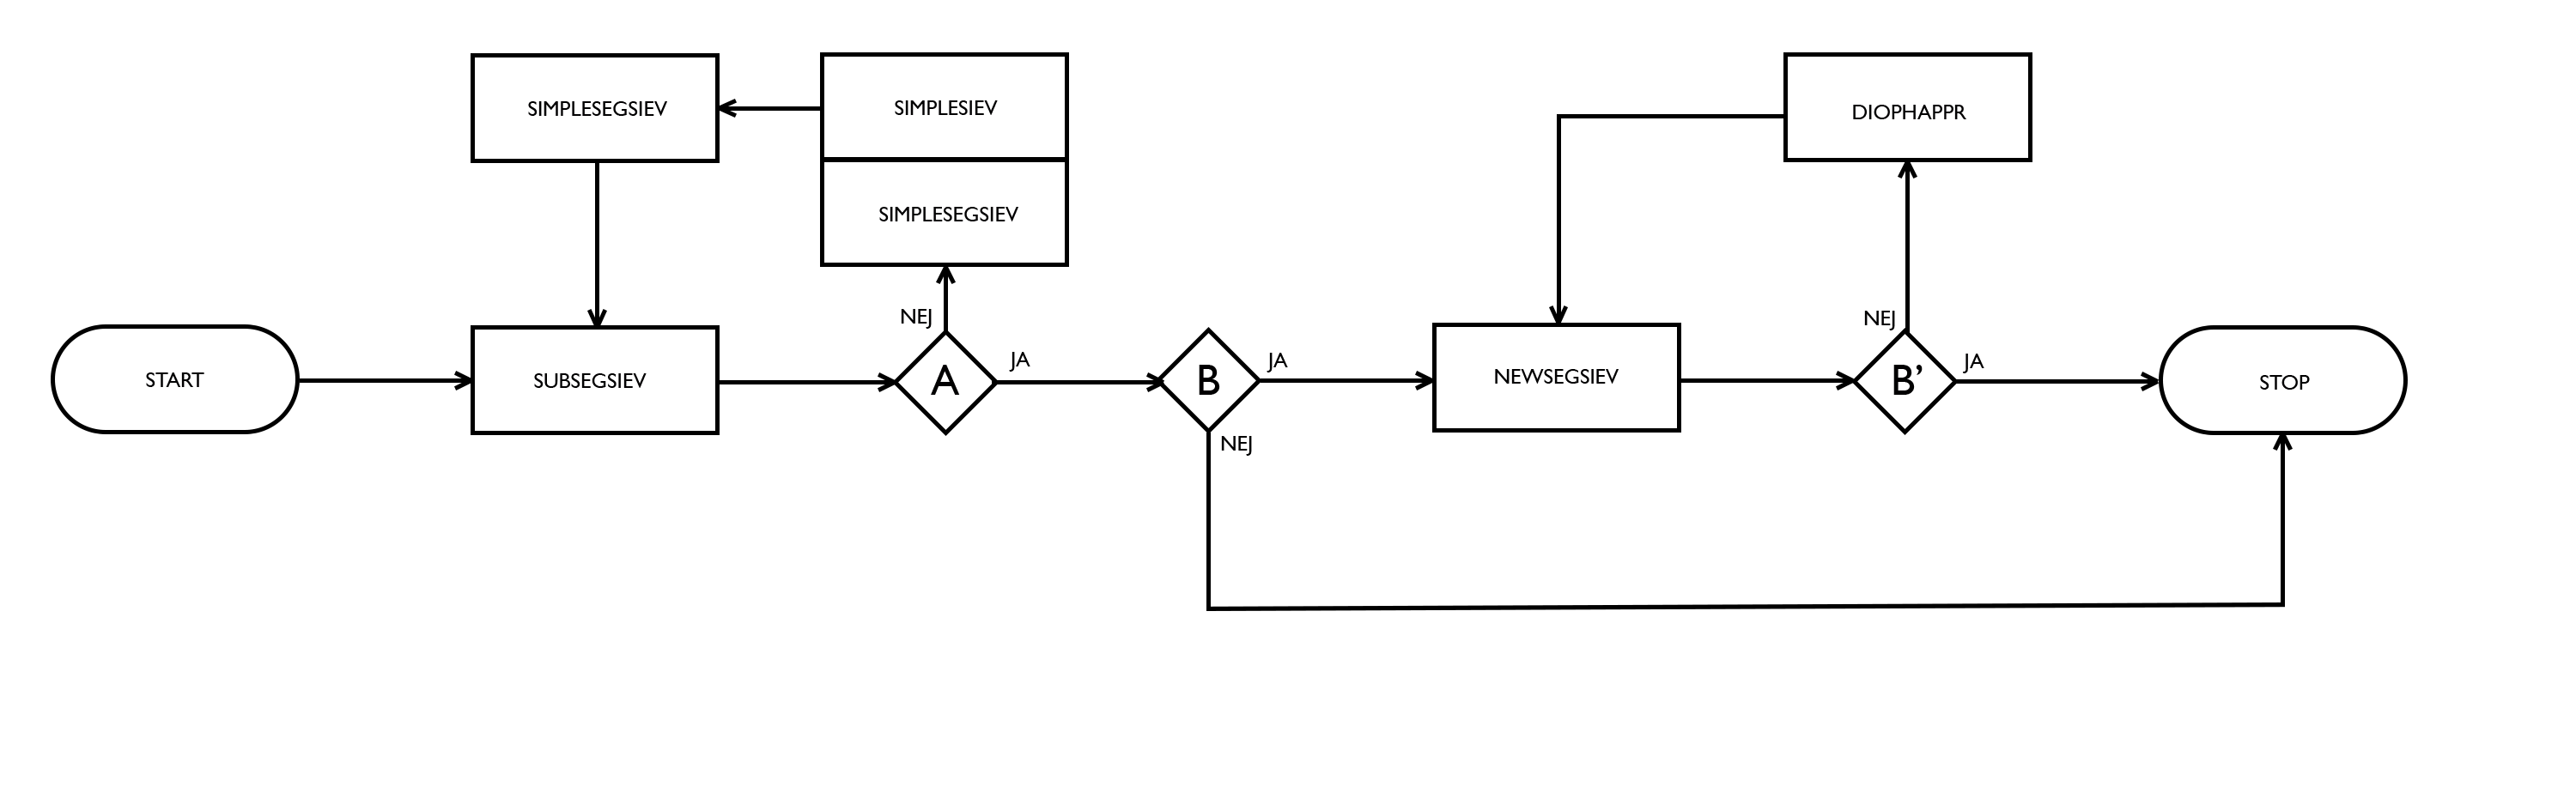
\includegraphics[width = \textwidth]{erik/Images/flowchart_v2.1.png}
    \usetikzlibrary{shapes.geometric, arrows, positioning}


\def\H{0.9cm}       % Min height for all objects
\def\W{2.15cm}      % Min width of rectangles
\def\Wpill{1.6cm}   % Min width of pills
\def\Wsplit{2.15cm} % Min width for split box (ugly solution)
\def\distV{1.4cm}   % Vertical distance between objects
\def\distH{0.6cm}   % Horizontal distance between objects


% Style
%\tikzstyle{every node} = [font=\tiny]
\tikzstyle{every node} = [font=\scriptsize]
\tikzstyle{every path} = [thick]
\tikzstyle{arrow} = [thick,->,>=stealth]

% Objects
\tikzstyle{startstop} = [rectangle, minimum width=\Wpill, minimum height=\H, text centered, draw=black, rounded corners=\H/2]
\tikzstyle{process}   = [rectangle, minimum width=\W, minimum height=\H, text centered, draw=black]
\tikzstyle{decision}  = [diamond,   minimum width=\H, minimum height=\H, text centered, draw=black]


{\fontfamily{qhv}\selectfont % phv, qhv eller qag 
\begin{tikzpicture}
% Objects
    % Start
    \node (start) [startstop]                       {\textsc{start}};
    % First loop
    \node (sub)   [process,  right=\distH of start] {\textsc{SubSegSiev}};
    \node (sim2)  [process,  above=\distV of sub]   {\textsc{SimpleSegSiev}};

    \node (sim1)  [process,  right=\distH of sim2, minimum width=\Wsplit]  {\textsc{SimpleSiev}};
    \node (sim0)  [process,  below=-\pgflinewidth of sim1, minimum width=\Wsplit]  {\textsc{SimpleSegSiev}};
    \node (A)     [decision, below=\distV of sim1]  {\textbf{A}};
    % Middle
    \node (B0)    [decision, right=\distH + 0.5cm of A]     {\textbf{B}};
    % Second loop
    \node (new)   [process,  right=\distH of B0]    {\textsc{NewSegSiev}};
    \node (B1)    [decision, right=\distH of new]   {\textbf{B'}};
    \node (dio)   [process,  above=\distV of B1]    {\textsc{DiophAppr}};
    % Stop
    \node (stop)  [startstop,right=\distH of B1]    {\textsc{stop}};

% Arrows
    % Start to first loop
    \draw [arrow] (start) -- (sub);
    % First loop
    \draw [arrow] (sub)   -- (A);
    \draw [arrow] (A)     -- (sim0);
    \draw [arrow] (sim1)  -- (sim2);
    \draw [arrow] (sim2)  -- (sub);
    % Middle
    \draw [arrow] (A)     -- (B0);
    \draw [arrow] (B0)    -- (new);
    \draw [arrow] (B0)    |- ([yshift=-\distV]B0.south) -| (stop);
    % Second loop
    \draw [arrow] (new)   -- (B1);
    \draw [arrow] (B1)    -- (dio);
    \draw [arrow] (dio)   -| (new);
    \draw [arrow] (B1)    -- (stop);

% Decision texts
    \node[above=3pt of A,  anchor=east]  {NEJ};
    \node[right=4pt of A,  anchor=south] {JA};
    \node[below=3pt of B0, anchor=west]  {NEJ};
    \node[right=4pt of B0, anchor=south] {JA};
    \node[above=3pt of B1, anchor=east]  {NEJ};
    \node[right=4pt of B1, anchor=south] {JA};
\end{tikzpicture}
}
\vspace{0.5cm}
    \caption{Ett övergripande flödesschema för algoritmen \textsc{NewSegSiev}. Observera att det finns två huvudloopar i algoritmen, en där kriterium A är uppfyllt då intervallet \([n - \Delta, n + \Delta]\) sållats med alla primtal \(p \leq K \Delta\) och den andra där kriterium B' är uppfyllt då algoritmen sållat för resterande tal upp till \(\sqrt{n + \Delta}\). Slutligen är kriterium B i koden identiskt med B' men illustrerar i flödesschemat möjligheten för programmet att aldrig gå in i den andra loopen då \(\Delta > \sqrt{n + \Delta}/K\).}
    \label{fig:flowchart}
\end{figure}


%Målet med \textsc{SubSegSiev} är att, givet \(n, \Delta \) och $M$, sålla \([n, n + \Delta]\) med primtal $p \leq M$. Algoritmen gör detta på i stort sett samma vis som i Eratosthenes klassiska såll men delar in primtalen i segment för att optimera minneskomplexiteten. \todo{Fortsätt med att gå igenom SimpleSiev, SimpleSegSiev och SubSegSiev och kort förklara hur de samverkar i NewSegSiev}.

Nästa steg, huvudalgoritmen i \textsc{NewSegSiev}, kräver mer matematisk eftertanke. Uppgiften som kvarstår för funktionen efter \textsc{SubSegSiev} är att sålla intervallet \([n - \Delta, n + \Delta]\) med resterande primtal, \( p \geq K \Delta\) där \(K \geq 5/2\). Problemet är löst genom att leta efter alla multiplar av \(m \geq K \Delta\) i vårt intervall. Låt \(\ell m\) vara en sådan multipel, då ser vi att
\begin{align} \label{alg.problem}
    n - \Delta \leq \ell m \leq n + \Delta \Longleftrightarrow 
    - \frac{\Delta}{m} \leq \frac{n}{m} - \ell \leq \frac{\Delta}{m} \Longleftrightarrow \left\{ \frac{n}{m} \right\} \in \left[- \frac{\Delta}{m}, \frac{\Delta}{m} \right] \bmod 1,
\end{align}
där $\big[- \frac{\Delta}{m}, \frac{\Delta}{m} \big] \bmod 1 = \bigcup_{k \in \mathbb{Z}} \big[k - \frac{\Delta}{m}, k + \frac{\Delta}{m} \big]$. Med den här presentationen av problemet gör \cite{HaraldSieve} två approximationer -- först en Taylorutveckling och därefter en diofantisk approximation. 

Den första approximationen syftar till att ersätta hyperbeln \(f(m) := \frac{n}{m}\) med en (diskontinuerlig) mängd tangenter till kurvan givna av en Taylorapproximation vid olika punkter \(m_0\),
\begin{align*}
    f(m) = f(m_0 + r) = \frac{n}{m_0} - \frac{n}{m_0^2} r + O\left(\frac{n}{m_-^3} r^2 \right)
\end{align*} % mellansteg nödvändigt?
där \(m_- = \min(m, m_0)\). Eftersom hyperbeln planar ut för större $m$ så kan vi approximera större och större intervall av kurvan med samma linjesegment utan att förstora feltermen. Mer specifikt så låter \cite{HaraldSieve} approximera kurvan med tangenter till kurvan på mitten, $m_0$, av intervallet \([M_i, M_i + 2R_i]\) där  $M_{i + 1} = M_i + 2R_i + 1$ med $M_0 = \lfloor K \Delta \rfloor + 1$ och
\begin{align*}% Eventuellt i stycke?
    R_i = \left\lfloor \sqrt{\Delta/(4n)} M_i \right\rfloor .
\end{align*}
Vi delar in kurvan i segment \([M, M + 2R]\) tills vi har täckt alla tal \(m \in [  \lfloor K \Delta \rfloor + 1, \sqrt{n + \Delta}]\). Orsaken till att \cite{HaraldSieve} väljer att definiera \(M, m_0\) och \(R\) som ovan är så att restermen inte övertar storleken på intervallet, med andra ord är resttermen \(\lesssim nr^2/m_-^3 \leq nR^2/M^3 = \Delta / (4M)\). Tar vi hänsyn till feltermen i problemformuleringen, (\ref{alg.problem}), så har vi omformulerat problemet till att hitta \(r \in [-R, R]\) så att \(P(r) = (\frac{n}{m_0} - \frac{n}{m_0^2} r) \in [-5\Delta/(4M), 5\Delta/(4M)] \bmod{1}\). Helfgotts val av \(K \geq 5/2\) fyller nu två syften: \(R \geq 1\) så att intevallen vi söker i inte är tomma och \(5\Delta/(4M) < 1/2\) så att intervallet vi försöker pricka inte är hela \(\mathbb{R}\).

Vi kan ställa ytterligare krav på \(r \in [-R, R]\) för att slippa gå över hela intervallet. Vad \cite{HaraldSieve} gör är att hitta en approximation för \(\alpha_1 := -n/m_0^2\) på formen \(a/q\) där $a,q$ är två relativt prima heltal med ett krav på nämnaren, $q \leq 2R$. Detta är precis funktionen av en så kallad diofantisk approximation och för att förstå den här processen krävs förkunskaper om kedjebråk som kan hittas i appendix \ref{APDX:cfrac}. Med kedjebråksnotationen från appendix så vill vi omformulera \(\alpha_1\) till ett enkelt kedjebråk, \(\langle a_0, a_1, \dots \rangle\). Följer vi algoritmen i \cite[sats 21.5]{Lindahl} så ges \(a_0\) av \(\lfloor \alpha_1 \rfloor\) och om inte \(\alpha_1\) var ett heltal, i vilket fall vi är färdiga, så blir resten \(0 < \alpha_1 - a_0 < 1\). Detta ger oss \(\xi_1 := 1 / (\alpha_1 - a_0) > 1\) och vi kan återupprepa samma steg: låt \(a_1 = \lfloor \xi_1 \rfloor\) och \(\xi_2 := 1 / (\xi_1 - a_1) > 1\). På så vis, om vi fortsätter, får vi en algoritm som genererar ett enkelt kedjebråk. 

%Det är förstås viktigt att veta att algoritmen har ett slut och för att se detta studerar vi konvergenterna \(c_n = p_n / q_n\). 
Vi kan vara säkra på att algoritmen slutar av sig självt eftersom vi utvecklar kedjebråket av ett rationellt tal, \(\alpha_1 = - n / m_0^2\), som därav är ett ändligt kedjebråk (se \cite[sats 21.5]{Lindahl}) men vi vill sannolikt avbryta processen redan tidigare. Vårt mål är att hitta en rationell approximation till \(\alpha_1\) med nämnare \(q \leq 2R\) och eftersom \((q_n)_{n>0}\) är en växande följd så kan vi välja att stoppa algoritmen när \(q_n \leq 2 R\) men \(q_{n + 1} > 2R\). Del 2 av sats \ref{app.kovfel} garanterar att vår approximation blir bättre för varje iteration och, för sådant $n$, så är \(\abs{\alpha_1 - \frac{a}{q}} \leq \frac{1}{q \cdot 2R}\). Till sist observerar vi att konvergenterna, \(p_n, q_n\), är relativt prima då del 2 av sats \ref{app.konvergenter} ger oss att \((p_{n-1}, q_{n-1})\) är en heltalslösning till den diofantiska ekvationen
\begin{align*}
    a x + b y = 1 \quad \text{ där }\ a = \pm q_n, b = \mp p_n
\end{align*}
vilket endast är möjligt om \(1\) är en multipel av största gemensamma nämnaren, \(\gcd{a,b}\), (ett resultat från elementär talteori, se förslagsvis \cite[sats 3.1]{Lindahl}). % H.L. istället för 1:a

Ovanstående algoritm heter \textsc{DiophAppr} i \cite{HaraldSieve} vilken beräknar en diofantisk approximation \(a / q\) av den ledande koefficienten \(\alpha_1\) i \(P(r)\) med kravet på $q$ som vi nämnde tidigare. Algoritmen returnerar täljare och nämnare separat samt passar på att beräkna \(a^{-1} \pmod{q}\) då del 2 av sats \ref{app.konvergenter} ger oss en möjlighet att räkna ut inversen i termer av konvergenterna. 

Målet med att introducera \textsc{DiophAppr} är så att vi kan gå från att leta lösningar till (\ref{alg.problem}) i \(r \in [-R, R]\) till att endast leta bland ett urval av heltal. Vi har redan hittat en rationell approximation av \(\alpha_1\) och, konstantkoefficienten av \(P(r)\), \(\alpha_0 := n / m_0\) kan vi också approximera med bråket \(\lfloor \alpha_0 q + 1/2 \rfloor / q := c / q\). Således ser vi att
\begin{align*}
    \abs{q \cdot P(r) - (c + ar)} &= \abs{\left(\alpha_1 - \frac{a}{q}\right) q r + \left( \alpha_0 q - c\right)} \leq 
    \abs{\alpha_1 - \frac{a}{q}} q \abs{r} + \abs{\alpha_0 q - c} \\
    &\leq \frac{1}{q \cdot 2R} \cdot qR + \frac{1}{2}  = 1
\end{align*}
tack vare noggrannheten av den diofantiska approximationen, hur vi definierade \(c\) och att \(r \in [-R, R]\). Därav, om \(P(r) \in [-5\Delta/(4M), 5\Delta/(4M)] \bmod 1\) så medför det att
\begin{align*}
    c + ar \in \{- k - 1, - k, ... , k, k + 1\} \bmod q
\end{align*}
där \(k = \lfloor q \cdot 5\Delta/(4M) \rfloor\). Det räcker alltså att sålla för \(r \equiv - a^{-1} (c + j) \pmod{q}\) för heltal \(j \in [-k-1, k+1]\), där den multiplikativa inversen av $a \pmod{q}$ tillhandahålls av \textsc{DiophAppr}. 

% Detta kan ge falska lösningar, vi kan kontrollera detta --> villkor på display-rad
Vi har alltså sett hur \cite{HaraldSieve} först sparar minnesplats genom att segmentera första delen av algoritmen och sedan tid i andra delen genom att vara selektiv med vilka tal som vi sållar bort multiplar av. I det senare fallet finns som mest en multipel i intervallet, per konstruktion av \(K \Delta\), och vi har visat att alla \(m = m_0 + r\) med en multipel i intervallet har \(r \equiv - a^{-1} (c + j) \pmod{q}\), för \(a, c, j\) definierade ovan. Däremot har vi inte visat det motsatta och det kan vara så att vissa \(r\) som genereras är falska lösningar orsakade av Taylor- och den diofantiska approximationen. Därför behöver vi också kontrollera att multipeln av \(m\) ingår i intervallet, det vill säga att
\begin{align} \label{alg.control}
    \ell m %:= \lfloor (n + \Delta) / m \rfloor \cdot m 
    \in [n - \Delta, n + \Delta] \quad \text{och } \quad  \ell m > m.
\end{align}

I nästa avsnitt kommer vi se vilka val som gick in i Python-implementationen av pseudokoden samt studera tidsbesparingar och möjliga förbättringar från originalalgoritmen.

%till den diofantiska approximationen \(a/q\) för \(\alpha_1\) så att \(\abs{\alpha_1 - \frac{a}{q}} \leq \frac{1}{q \cdot 2R}\) för största möjliga konvergent $q$ mindre än eller lika med \(2R\). \textsc{DiophAppr} 

\subsection{Vår implementering}
% Skrivet av Nils

Algoritmerna i \cite{HaraldSieve} presenteras i form av pseudokod som för att kunna användas, måste översättas till något programmeringsspråk.
Vår implementation av algoritmerna är skrivna i språket Python.
%Vi har valt att använda språket Python för att implementera algoritmerna.
Det var möjligt att översätta pseudokoden mer eller mindre ordagrant, vilket gjordes och resulterade i en första version av programmet.
Därefter kunde flera förbättringar av koden göras för att korta ned dess körningstid. 
Vissa av förbättringarna var möjliga då pseudokoden i \cite{HaraldSieve} är skriven i syfte att tydligt illustrera algoritmerna,
och är således inte ämnad till att vara färdig, optimerad kod.
Andra förbättringar var språkspecifika och åstadkoms genom att jämföra beräkningstiden hos olika funktioner och metoder i Python, för att sedan implementera de som visade sig vara snabba.
Den förbättrade versionen av koden finns bifogad i appendix.
Nedan följer, utan inbördes ordning, några av de gjorda förbättringar som har haft större inverkan.
\begin{myitemize}
    \item
    I den ursprungliga pseudokoden representeras den sållade mängden av en vektor bestående av booleaner, vilken vi har ersatt med en bitsträng.
    %Algoritmen sållar primtal ur en lista som i det ursprungliga programmet representeras av en vektor bestående av booleaner.%  Det ursprungliga programmet sållar över en vektor av booleaner, vilken vi har valt att ersätta med en bitsträng.   
    %Istället för att spara och göra beräkningar på en vektor av booleaner, väljer vi att uttrycka mängden som en bitsträng. 
    Denna idé föreslås redan i \cite{HaraldSieve} och sparar i första hand minne,
    som i sin tur kan leda till snabbare beräkningar på grund av bättre användning av cache.
    Här användes Python-biblioteket \textit{Bitarray}.
    \item
    På vissa ställen har det varit möjligt att flytta ut beräkningar utanför loopar så att samma beräkning inte behöver göras flera gånger. 
    Dessutom har flera beräkningar kunnat kortas ned eller skrivas ihop för att undvika temporära variabler.
    \item
    I Python kan operatorn \texttt{x//y} användas för division utan rest. Denna har visat sig vara snabbare än sammansättningen \texttt{floor(x/y)} och har därför fått ersätta den senare där det varit möjligt. På ett liknande sätt har \texttt{ceil(x/y)} ersatts med \texttt{-(x//-y)}.
\end{myitemize}

%En ytterligare förbättring kunde göras efter en noggrann analys av pseudokoden för \textsc{NewSegSiev};
%Efter diofantisk approximering erhålls $n'\geq0$, en multipel av $m>0$ som möjligen uppfyller $n'\in[n-\Delta,n+\Delta]$ och $n'>m$.
En ytterligare förbättring kunde göras genom att titta närmare på (\ref{alg.control}).
För att en lösning $m$ ska vara en äkta lösning måste alla villkor i (\ref{alg.control}) hålla
och detta bör således kontrolleras i algoritmen.
Men i själva verket är det överflödigt att kontrollera alla tre villkoren.

Algoritmen konstruerar nämligen multipeln $\ell m$ genom att sätta $\ell:=\lfloor (n+\Delta)/m \rfloor$,
vilket direkt implicerar att $\ell m \leq n+\Delta$ alltid är uppfyllt.
Vidare inspekterar vi villkoret $\ell m>m$, där vi har att
\begin{equation*}
    \ell m>m \iff
    \left\lfloor \frac{n+\Delta}{m} \right\rfloor > 1 \iff
    \left\lfloor \frac{n+\Delta}{m} \right\rfloor \geq 2 \iff
    (n+\Delta)/2\geq m.
\end{equation*}
Men $m$ väljs ur intervallet $[M,M+2R]$ så det räcker med att undersöka vilka förhållanden som  $M+2R\leq(n+\Delta)/2$ är uppfyllt under:
Vi har att $M\leq\sqrt{n+\Delta}$, $R=\lfloor M\sqrt{\Delta/4n}\rfloor$ samt $\Delta\leq n$ vilket ger oss att $M+2R \leq 2\sqrt{n+\Delta}$.
Detta är i sin tur mindre eller lika med $(n+\Delta)/2$ om $n+\Delta\geq16$.
Att sålla efter primtal i en lista av positiva heltal mindre än $16$ är ointressant.
Därför kan vi rimligtvis introducera kravet $n+\Delta\geq16$ i början av \textsc{NewSegSiev},
så att $\ell m>m$ alltid håller och därmed inte behöver testas senare i algoritmen.

Det har följaktligen visat sig att av de tre villkor i (\ref{alg.control}),
är två av dem alltid uppfyllda och behöver därmed inte kontrolleras.
Det totala antalet gånger som detta steg utförs är
\begin{equation*}
    O\left(\Delta\log n + \sqrt{n/\Delta}(\log n)^2\right),
\end{equation*}
enligt \cite[s.346]{HaraldSieve} och vi sparar således en betydande mängd tid på att reducera antalet beräkningar här till en tredjedel av det ursprungliga.


För att visa att de förändringar som gjorts i koden, faktiskt har haft inverkan så lät vi utföra tester.
Testerna gjordes på en hemdator och jämförde körningstid mellan den första versionen av programmet, mot en senare version där förbättringarna har införts.
Som tidigare nämnts så sållar algoritmen fram primtal i ett angivet intervall $[n-\Delta,n+\Delta]$ och 
dess tillvägagångssätt varierar något beroende på förhållandet mellan $\Delta$ och $n$.
Av denna anledning utfördes två stycken tester där detta förhållande sattes till att vara så stort som möjligt respektive så litet som möjligt.
I det första testet valdes således $\Delta:=n$ och tre mätningar utfördes för $n=5\cdot10^3,5\cdot10^5,5\cdot10^7$.
I det andra testet valdes $\Delta:=\sqrt[3]{n}$ och $n$ fick anta värdena $10^9$, $10^{12}$ respektive $10^{15}$.
För alla mätningar visade sig den förbättrade versionen vara minst 10 gånger så snabb som den ursprungliga versionen, dessutom visar mätningarna på en antydan till att denna faktor ökar då $n$ växer. De uppmätta tiderna finnes i tabell \ref{implementering.tidtabell}.



Givetvis är programmet inte perfekt och det finns flera knep som kan utforskas ifall ytterligare förbättring av koden eftertraktas.
I den ursprungliga artikeln \cite{HaraldSieve} nämns ett fåtal eventuella förbättringar, här ges ytterligare två stycken.
\begin{myitemize}
    \item
    Istället för att flera gånger om låta \textsc{SimpleSiev(M)} generera en lista med alla primtal upp till $M$ kan det eventuellt spara tid att generera en godtycklig lista vid start av programmet.
    Värdet på $M$ överskrider inte $\sqrt{K\Delta+\sqrt{K\Delta}}$, vilket gör denna taktik rimlig.
    Exempelvis tar en lista med alla primtal upp till en miljard omkring 1GB att spara och kan användas för $n\leq 10^{35}$, så länge som vi håller oss till något mindre interval där $\Delta\leq\sqrt{n}$.
    Detta handlar självklart om en avvägning mellan hur snabbt det går att läsa in sparad data mot hur snabbt det går att beräkna den från grunden och bör undersökas mer innan idén tillämpas.
    \item
    Flera beräkningar kan utföras parallellt, vilket redan föreslås i \cite{HaraldSieve}. 
    I synnerhet kan detta nyttjas i andra delen av \textsc{NewSegSiev} där oberoende beräkningar utförs för varje $j\in[-k-1,k+1]$.
    Dessa beräkningar är alla enkla och på samma form, och det kan således vara gynnsamt att överlåta dessa till datorns grafikkort.
    Detta eftersom grafikkortet ofta visar sig snabbare än processorn på att utföra denna typ av uppgifter.
\end{myitemize}



\begin{table}[h]
\centering
\caption{
Uppmätta körningstider för den första, respektive den förbättrade versionen av programmet.
Programmet sållade fram alla primtal i ett intervall på formen $[n-\Delta,n+\Delta]$ där $\Delta=n$ för de tre första mätningarna och $\Delta=\sqrt[3]{n}$ för de tre sista.
Den förbättrade versionen var snabbare än den första versionen med en faktor på minst 10, för alla mätningar.}
\renewcommand{\arraystretch}{1.3} % Changes height of each row

\begin{table}[H]
\begin{center}
\begin{tabular}{|c||r|r|}
    \hline
    \multirow{2}{*}{\ Intervall\ } & \multicolumn{2}{c|}{Körningstid (s)}\\
    \cline{2-3}
    & Utan förbättringar & Med förbättringar\\
    \hline
    $\left[0,10^{6}\right]$ & 0.00534 & 0.000534\\
    $\left[0,10^{9}\right]$ & 0.00534 & 0.000534\\
    $10^{9}\pm 10^{3}$ & 0.00534 & 0.000534\\
    $10^{12}\pm 10^{4}$ & 0.00534 & 0.000534\\
    \hline
\end{tabular}
\end{center}
\label{implementering.tidtabell}
\caption{Körningstider för den första versionen, respektive den förbättrade versionen av programmet. Intervallen har valts till...}
\end{table}

\label{implementering.tidtabell}
\end{table}

I nästkommande avsnitt presenteras diverse resultat som erhållits ifrån körning av programmet.



\begin{comment}
    \item
    Deklaration av temporära variabler har i vissa fall kunnat uteslutas genom sammanskrivning av flera uttryck. 
    Ett specialfall av detta nyttjas i \textsc{DiophAppr} där vi har ersatt uttryck på formen \texttt{temp=x; x=y; y=temp;} med det snabbare \texttt{x,y=y,x;}.

    \item Flera while-loopar har kunnat ersättas med for-loopar,
    som ger att istället för att testa ett argument för varje iteration i loopen,
    behöver argumentet bara testas en gång när loopen påbörjas.
    \item Infogande av iteratorer vid iterering över primtalslistor, vilket också resulterar i bättre nyttjande av cache.

    \item
    I \textsc{DiophAppr} beräknas både heltals- och decimaldelen av $\alpha$. Detta görs i nuläget separat men skulle kunna göras samtidigt.
    Förslagsvis skulle då if-satsen ändras till att testa ifall decimaldelen är noll.
\end{comment}

\subsection{Tillämpningar och resultat}
\todo{Introducera de tillämpningar som ska tagits upp; enkla primtal, tvillingsprimtal, primtal i aritmetiska talföljder, storleken på primtalsgap(?).}

%Over the course of this report we have refered to ,and approximated, the distribution of variouss classifications of prime numbers. Using now our implementation of Helfgott's origianl code we seeek to present the legitimacy of said distributions and also reflect on the quality of the code which we have written. The specific distributions ot be presented are those of the regula r prime numbers, the twin primes, as well as primes in arithmetic sequences. For each of these distributions have slight modifications been made to the code, which will be briefly discussed.

\subsubsection{Fördelningen av primtal}
\todo{Grafera antalet primtal vi har hittat jämfört emot PNT, både x/log x och Li(x). Diskutera sedan varför skillnader finns/ vad för slutsats vi kan dra(?)/ hur vi har kommit här?}
%Beginning with the classic example of the set of prime numbers, below is illustrated the distribution predicted by the familiar x over log x from sieve theory/Chebychev, the more accurate lorgarithmic integral Li(x), and the actual number of primes found in using our implementation. In order to generate the following graph, no new sieving methods were introduced, simply the counting fucntion in Appendix X
\begin{figure}[H]
    \centering
    
\includegraphics[width = 0.7\textwidth]{coen/Images/test.png}
    \caption{\todo{Infoga en graf med antalet primtal enligt koden, x/log x, och Li(x)}}
    %This graph shows the relative distributions of primees as per the aforementioned fucntions. Notice that while x over log x appears relatively close for smaller x the logarithmic integral approximation is a near exact match for the true distribution, so much so that the code line is hidden.
    \label{fig:res.prime}
\end{figure}
%As shown in figure X, should we believe in the PNT it seems as though our code does indeed find the correct number of primes. The rather large error in the x over log x estimate is indicative/reflective of one of the limitations highlighted in Section XXX, namely the impact of the error terms and their reconcillation with the main terms. Howeve, there doest exist a deeper link between the x over log x estimate and that of the logarithmic integral. Throguh the use of integral wizardry you can decompose the logarithmic integral into a series of terms, the first of which being x over log x with the remainder being of the order of sqrt(x). This then accounts for the increase in error as x grows. Thiese kinds of approximations for the prime counting function can also be rather naturally extrapolated to those for twin primes, as discussed below.

\subsubsection{Fördelningen av tvillingsprimtal}
\todo{Introducera de förändringarna som utfördes för att tillåta koden att sålla efter tvillingsprimtal.}
%Continuing our presentation of various sets of prime's distributions, next we turn to the other recurring theme of twin primes. The following figure illustrates the distributions of twin primes as predicted by x over log squared x and the second order logarithmic integral against those primes found using our implementation. It should be noted that a rather simple help function, Appendix XXX, was written which searches for non twin primes in the prime list and removes them.
\begin{figure}[H]
    \centering
    
\includegraphics[width = 0.7\textwidth]{coen/Images/test.png}
    \caption{\todo{Infoga en graf med antalet tvillingsprimtal enligt koden, Cx/log2 x, CLi\textunderscore2(x), undre begränsningen som finns i rapporten. Ge en motivation till varför C är vad det är och vartifrån fördelningen kommer.}}
    %This graph shows the relative distributions of the twin primes as per the aforementioned fucntions. Notice once again the accuarcy of the logarithmic integral, once again hiding our code line, as opposed to that of C x over log squared x, where the constant is 2*C_2, or 2 times the twin prime constant (discussed below).
    \label{fig:res.twins}
\end{figure}
\todo{Diskutera och förklara varför saker ser ut som de gör, vanliga saker. Kan vi lita på koden?(Kanske inte nödvändigt)}
%There are a number of things to discuss regardng the above figure. 
\subsubsection{Fördelningen av primtal i aritmetiska talföjlder}
\todo{Introducera de förändringarna som utfördes för att tillåta koden att sålla efter primtal i vissa aritmetiska talföljder.}
\begin{figure}[H]
    \centering
    
\includegraphics[width = 0.7\textwidth]{coen/Images/test.png}
    \caption{\todo{Infoga en graf med antalet primtal i aritmetiska följder enligt koden, Brun-Titchmarsh, Dirichlet serier(eller vad det nu var). Vad har vi valt epsilon till? Gör det något skillnad?}}
    \label{fig:res.arit}
\end{figure}
\todo{Diskutera ovanstående graf. Hur rimligt är uppskattningen? Hur dåligt är vår bästa approximation enligt koden?}


%\section{Metod och genomförande}
%% Skrivet av Nils

Denna rapport är framför allt en litteraturstudie, med stor förankring i \textit{An Introduction to Sieve Methods and Their Applications} av Alina Carmen Cojocaru \& M. Ram Murty (2005). Rapporten ämnar \textbf{att introducera matematikstudenter på sen kandidatnivå till sållteori.} Vi presenterar tre stycken såll som har haft stor teoretisk och historisk betydelse för ämnet och exemplifierar dessa i programmeringsproblem. 

I teoridelen formuleras de mest centrala satserna och idéerna men bevisen har i vissa fall kortats ned och i andra fall helt överlåtits till appendix, detta i syfte att göra texten mer lättillgänglig för läsaren.



%\begin{thebibliography}{FFF}
%\bibitem[UR]{rapp} Utformning av rapporter och kandidatarbetens skriftliga presentation för Civilingenjörsprogrammen vid Chalmers tekniska högskola. 2008. Göteborg: Chalmers Tekniska Högskola

\newpage
\printbibliography

%\end{thebibliography}
\medskip

\newpage
\appendix
\section{Ordonotation}
I den här uppsatsen gör vi flitig användning av ordonotation för att beteckna olika asymptotiska gränser. För $D \subset \mathbb{C}$ och två funktioner, $f: D \to \mathbb{C}$ och $g: D \to \mathbb{R}_+$ skriver vi
\begin{align*}
    f(x) = O(g(x)) \quad \text{om det finns } A > 0 \text{ så att} \quad \abs{f(x)} \leq A g(x), \forall x \in D.
\end{align*}
Omväxlande skriver vi även \(f(x) \ll g(x)\) med samma betydelse som ovan. Om vi har att \(f(x) \ll g(x)\) och \(g(x) \ll f(x)\) så skriver vi \(f(x) \asymp g(x)\).
\section{Partiell summation}
\section{Ett lemma angående multiplikativa funktioner}
Följande lemmat är hämtad från \cite[Lemma 7.2.2]{cojocarumurty}, där beviset utelämnas.
\begin{lemma}\label{APDX:multFunk}
Låt \textit{f} vara en multiplikativ funktion med \(d_1,d_2\) positiva, kvadratfria heltal. Då
\begin{equation}
    f([d_1,d_2])\cdot f((d_1, d_2)) = f(d_1)f(d_2)\nonumber
\end{equation}
\end{lemma}
\begin{proof}
Vi delar upp beviset i två fall där \(d_1\) och \(d_2\) är antingen relativt prima eller inte. Då \(d_1\) och \(d_2\) är relativt prima är \((d_1,dd_2) = 1\) och \([d_1,d_2] = d_1d_2\). Detta medför att
\begin{equation}
    f([d_1,d_2])\cdot f((d_1, d_2)) = f(d_1d_2)f(1) = f(d_1)f(d_2)\nonumber
\end{equation}
där sista likheten gäller för att  \(d_1\) och \(d_2\) är relativt prima. 

Då  \(d_1\) och \(d_2\) inte är relativt prima är både deras lägsta gemensamma multipel och största gemensamma delare också kvadratfria. Genom att skriva \([d_1,d_2]\) och \((d_1,d_2)\) som
\begin{align}
    [d_1,d_2] &= p_1p_2...p_m\nonumber\\
    (d_1,d_2) &= q_1q_2...q_l\nonumber
\end{align}
och med användning av formeln \([d_1,d_2]\cdot(d_1,d_2) = d_1d_2\) har vi att
\begin{equation}
    f([d_1,d_2])\cdot f((d_1, d_2)) = f(p_1)f_(p_2)...f(p_m)f(q_1)f(q_2)...f(q_l) = f(d_1)f(d_2)\nonumber
\end{equation}
där i sista likheten kombinerar vi om de primtal som behövs för att få tillbaka \(d_1\) och \(d_2\), vilket vi kan göra på grund av formeln som nämndes tidigare.
\end{proof}
\section{Kedjebråk}


\end{document}                 % The input file ends with this command.
